\documentclass[11pt]{article}
\usepackage{amssymb}
\usepackage{mathtools}
\usepackage{algorithm}
\usepackage{listings}
\usepackage{multicol}
\usepackage[noend]{algpseudocode}
\usepackage[english]{babel}
\DeclarePairedDelimiter{\ceil}{\lceil}{\rceil}

% TikZ Drawing packages

\usepackage{bbm}
\usepackage{tikz}
\usepackage{pgfplots}
\usetikzlibrary{arrows}
\usetikzlibrary{automata,positioning}

\usepackage{hyperref}
\hypersetup{
    colorlinks=true,
    linkcolor=blue,
    filecolor=magenta,      
    urlcolor=cyan,
}

\lstset{
  frame=tb,
  language=python,
  tabsize=4,
  keywordstyle=\textbf,
  basicstyle={\small},
  breaklines=true
}

\textwidth=6in
\oddsidemargin=0.25in
\evensidemargin=0.25in
\topmargin=-0.1in
\footskip=0.8in
\parindent=0.0cm
\parskip=0.3cm
\textheight=8.00in
\setcounter{tocdepth} {3}
\setcounter{secnumdepth} {2}
\sloppy

\tikzset{
    ->, % makes the edges directed    
    node distance=5cm, % specifies the minimum distance between two nodes. Change if necessary.
    every state/.style={thick, fill=gray!10}, 
    initial text=$ $,
}

\begin{document}

\setlength{\oddsidemargin}{.25in}
\setlength{\evensidemargin}{.25in}
\setlength{\textwidth}{6in}
\setlength{\topmargin}{-0.4in}
\setlength{\textheight}{8.5in}

\newcommand{\handout}[4]{
   \noindent
   \begin{center}
   \framebox{
      \vbox{
    \hbox to 5.78in { {\bf Automatic Verification of Systems} \hfill #1 }
       \vspace{4mm}
       \hbox to 5.78in { {\Large \hfill #4  \hfill} }
       \vspace{2mm}
       \hbox to 5.78in { {\it #2 \hfill #3} }
      }
   }
   \end{center}
   \vspace*{4mm}
}

\newcommand{\finalProjTitle}[4]{\handout{#1}{Lecturer:
#2}{Names: #3}{#4}}

\newtheorem{theorem}{Theorem}
\newtheorem{corollary}[theorem]{Corollary}
\newtheorem{lemma}[theorem]{Lemma}
\newtheorem{observation}[theorem]{Observation}
\newtheorem{proposition}[theorem]{Proposition}
\newtheorem{definition}[theorem]{Definition}
\newtheorem{claim}[theorem]{Claim}
\newtheorem{fact}[theorem]{Fact}
\newtheorem{assumption}[theorem]{Assumption}
\newtheorem{example}{Example}

\newcommand{\qed}{\rule{7pt}{7pt}}

\newenvironment{proof}{\noindent{\bf Proof:}\hspace*{1em}}{\qed\bigskip}
\newenvironment{proof-sketch}{\noindent{\bf Sketch of Proof:}\hspace*{1em}}{\qed\bigskip}
\newenvironment{proof-idea}{\noindent{\bf Proof Idea:}\hspace*{1em}}{\qed\bigskip}
\newenvironment{proof-of-lemma}[1]{\noindent{\bf Proof of Lemma #1:}\hspace*{1em}}{\qed\bigskip}
\newenvironment{proof-attempt}{\noindent{\bf Proof Attempt:}\hspace*{1em}}{\qed\bigskip}
\newenvironment{proofof}[1]{\noindent{\bf Proof}
of #1:\hspace*{1em}}{\qed\bigskip}
\newenvironment{remark}{\noindent{\bf Remark}\hspace*{1em}}{\bigskip}

%%%%%%%%%%%%%%%%%%%%%%%%%%%%%%%%%%%%%%%%%%%%%%%%%%%%%%%%%%%%%%%%%%%%%%%%%%%%%%%%%%%%%

\title{\vspace{-2.0cm}\textbf{Automatic Verification of Systems \\ Final Project - 
Symbolic Model Checker}}
\author{
	Omri Lifshitz \\
	\texttt{205490675} \\
	\texttt{omrilifshitz@mail.tau.ac.il}
	\and 
	Idan Berkovits \\
	\texttt{205404130} \\
	\texttt{berkovits@mail.tau.ac.il}
}
\date{}

\maketitle

%%Michal%% ==> Change the lecture number, lecture date, and Scribe name
%\finalProjTitle{September 3, 2018}{Dr. Sharon Shoham}{Omri Lifshitz, Idan Berkovits}
%{Symbolic LTL Model checking}

\section{Abstract}

   In this project, we implement a symbolic LTL model checker, using the reduction to the fair-CTL verification
   problem. We compare between the CTL model checker and the LTL model checker and show that the LTL behaves
   exponentialy in the size of the model. We also extend the original tableau definition to test the impact
   on simple formulas that use the Global and Eventually quatifiers.

\section{Introduction}
   Throughout the course we studied LTL and CTL model checking and algorithms
   used to solve this problem. Though we thoroughly learned the theoretical 
   approach to the model checking problem and the algorithms used to solve them, we did not
   go into detail regarding the verifcation tools available to solve these problems.
   One verifcation tool that we came across during the course was the SMV model
   checker and its expansion to LTL formulae found in \cite{ltl}. Although the
   SMV model checker is a very useful tool for model checking, it is written
   in a pseudo-code language that is not very common to most programmer.
   
   In our project we created a new model checker in $python$ that allows
   verifcation of both temporal logics LTL and CTL. The model checker we
   implemented is symbolic in order to be efficient and uses the algorithms
   shown in class for model checking. Our intention was to create a model
   checker that is both efficeint and easy to use and expand. We have developed
   the relevant modules to simply translate a logical model $M$ into a symbolic
   representation and use this symbolic representation in order validate
   LTL and CTL formulae.
   We tested our model checker on the snooping cache coherence protocol as
   found in \cite{cache}. 
   
   In this paper we describe the relevant algorithms and theory needed to
   understand the implemenation of our model checker. We also describe the 
   main modules of the model checker and the results it achieved on the 
   cache coherence model.

   The entire implementation of this project can be found at \url{https://github.com/olifshitz/AutomaticVerification.git}

\section{CTL and LTL Model Checking}

   \subsection{CTL*, LTL and CTL}
        Let us begin by describing the temporal logic CTL*, and from there continue
        to describe both Computation Tree Logic (CTL) and Linear Temporal Logic(LTL).
        CTL* contains two types of formulae: state formulae which hold for specific
        states and path formulae which hold along a specific path. State formulae
        are given by the following rules \cite{ltl}:
        \begin{itemize}
            \item
                If $p \in AP$ (Atomic propositions) then $p$ is a state formula.

            \item
                If $f,\; g$ are state formulae then $\neg f, f \vee g$ are state formulae.

            \item
                If $f$ is a path formula, then $Ef$ ("for some computation path")
                is a state formula.
        \end{itemize}

        Path formulae are defined by the following rules:
        \begin{itemize}
            \item
                If $f$ is a state formula, it is also a path formula.

            \item
                If $f,\; g$ are path formulae then $\neg f,\; f \vee g, \; Xf$ and 
                $fUg$ are also path formulae.

            \item
                If $f$ is a path formula, then $Ef$ ("for some computation path")
                is a state formula.
        \end{itemize}
        
        Let $M = (S,R,L)$ be a Kripke structure where $S$ is the set of states, $R$
        is the transition relation (we assume there is a total transition relation)
        and $L$ be the labeling function.

        \begin{definition}
            A path in Kripke structure $M$ is an infinite sequence of states 
            $\pi = s_0,s_1,\dots$ such that for every $i\geq 0$, 
            $(s_i, s_{i+1})\in R$.
        \end{definition}

        The notation $M, s \models f$ is used to state that $f$ holds for state
        $s$ in the Kripke structure $M$, and similarly for $M, \pi \models f$ for
        path $\pi$ in $M$.

        \begin{definition}
            Let $f_1, f_2$ be state formulae and $g_1, g_2$ path formulae. 
            The relation $\models$ is defined recursively as follows:
            \begin{eqnarray}
                M,s \models p &\iff & p\in L(s) \\
                M,s \models \neg f_1 &\iff &M,s \not\models f_1 \\
                M,s \models f_1 \vee f_2 &\iff & M,s \models f_1 \text{or} M,s \models f_2 \\
                M,s \models Eg_1 &\iff &\text{there is a path $\pi$ starting at $s$ such
                that $M, \pi \models g_1$}\\
                M, \pi \models f_1 &\iff & s \text{ is the first state of $\pi$ and }
                M,s \models f_1 \\
                M, \pi \models \neg g_1 &\iff &M,\pi \not\models g_1\\
                M,\pi \models g_1 \vee g_2 &\iff & M,\pi \models g_1 \text{ or } M,\pi \models g_2 \\
                M, \pi \models Xg_1 &\iff &M,\pi^1 \models g_1\\
                M,\pi \models g_1Ug_2 &\iff &\exists k\geq 0\; s.t.\; M,\pi^k\models g_2\;
                \text{ and } \forall 0\leq j\leq k\; M,\pi^j \models g_1
            \end{eqnarray}
        \end{definition}

        \begin{definition}
            CTL is the subset of CTL* obtained by specifying the path formulae using
            the following rules\cite{ltl}:
            \begin{itemize}
                \item
                    If $f,\;g$ are state formulae, then $Xf$ and $fUg$ are path
                    formulae.
                \item
                    If $f$ is a path formulae, then so is $\neg f$.
            \end{itemize}
        \end{definition}

        From the definition we can see that CTL is a subset of CTL* that only permits
        branching operators. Therefore, in this new logic, all linear-time operators
        can only appear if they are immediately preceded by path quantifiers.

        \begin{definition}
            LTL is a subset of CTL restricted to all formulae of the form $Af$ where
            $f$ is a path formula in which the only state sub-formulae are atomic
            propositions\cite{ltl}.
            More precisely, path formulae here are defined in the following recursive
            manner:
            \begin{itemize}
                \item
                    An atomic proposition.
                \item
                    If $f,\; g$ are path formulae, then $\neg f,\; f\vee g,\;
                    Xf$ and $fUg$ are also path formulae.
            \end{itemize}
        \end{definition}


    \subsection{Symbolic CTL Model Checking}
        Let us first begin by describing the usage of reduced, ordered 
        binary decision diagrams (ROBDDs). The names BDD
        (binary decision diagrams) and ROBDDs will be used iterchangealy
        throughout the paper. BDDs are a canonical form representation of
        boolean formulas\cite{bdd}.

        BDDs are very similar to binary decision trees and hold the following
        properties:
        \begin{itemize}
            \item 
                The BDDs are directed acyclic graphs (DAG) rather than tree
                trees.
            \item
                There is a total order on the occurence of the variables in the
                BDD when transversing the diagram from the root to the leaf.

            \item
                Each subgraph represents a unique boolean formula.
            
            \item
                The BDD representation of a boolean formula is unique given
                a certain variable ordering.
        \end{itemize}

        BDDs are very efficient in boolean function representation and can be
        easily manipulated and thus can be very useful in model checking.

        The objective of CTL model checking is to find the set of states in a
        given model for which a CTL formula holds. Symbolic CTL model checking
        uses BDDs in order to represent the states int he model and its transitions.
        That is, the transition relation in the Kripke structure is given by
        a boolean formula $R(v,v')$ representing if there is a relation from the
        set of state $v$ to the set of states $v'$. For each subformula, the 
        algorithm computes the states satisfying it in a bottom up manner and returns
        a BDD that represents the relevant states.


    \subsection{LTL Model Checking Using Tableaus}
        As taught in class, and also shown in \cite{ltl}, we can use tableaus in
        order to perform LTL model checking. In this section we present the
        construction of the tableau and how to use in order to create the product
        model. We also explain how the product model can be used in order to 
        find every path that satisfies $f$ in formula $Ef$ givne model $M$.

        Let us begin by describing the tableau. Let $AP$ be the set of atomic
        propositions in formula $f$. We define the set of elementary formulae
        in the following inductive manner:
        \begin{itemize}
            \item 
                $el(p) = \left\{p\right\}$ if $p\in AP$

            \item
                $el(\neg g) = el(g)$

            \item 
                $el(g\vee h) = el(g) \cup el(h)$

            \item 
                $el(\mathbf{X}g) = \left\{\mathbf{X}g\right\} \cup el(g)$

            \item 
                $el(gUh) = \left\{X(gUh)\right\} \cup el(g) \cup el(h)$
        \end{itemize}

        From the elementary formulae defined above, we create the states of the
        tableau by looking at the states $2^{el(f)}$. The labeling function for
        the tableau gives each state the atomic propositions found in the 
        elementary formulae that makes up the state.

        We also define the set $sat(g)$ for each subformula $g$ to be the set of
        states that satisfy $g$. The set is defined in the following inductive
        manner:
        \begin{itemize}
            \item 
                $sat(g) = \left\{\sigma \; |\; g\in \sigma\right\}$ where
                $g \in el(f)$

            \item 
                $sat(\neg g) = \left\{\sigma \;|\; \sigma \not\in sat(g)\right\}$

            \item
                $sat(g\vee h) = sat(g) \cup sat(h)$

            \item
                $sat(g U h) = sat(h) \cup (sat(g) \cap sat(X(gUh)))$
        \end{itemize}

        The transition relation of the tableau is given by the following formula:
        \[
            R_T(\sigma, \sigma') = \underset{Xg\in el(g)}{\bigwedge}
                \sigma\in sat(Xg) \iff \sigma' \in sat(g)
        \]

        The transition relation above does not guarantee that the eventually
        property holds; for example in the case of the subformula $aUb$ - the
        transition relation leading to a path where $a$ always holds and $b$ is
        never reached is also valid. 
        
        In order to overcome this problem we need to add more conditions on the
        paths accepted by the tableau. We do this by adding the fairness 
        constraint matching the eventually property described above. 
        That is, for every subformula $gUh$, we add the fairness constraint
        \[
            \left\{sat(\neg(gUh)\vee h \;|\; gUh in f \right\}
        \]

        This concludes the construction of the tableau; we now move to describing
        the product model created from the tableau above, $T$ and the original 
        model $M$. The product is defined as the following Kripke structure:
        \begin{itemize}
            \item
                $S = \left\{(\sigma, \sigma')\;|\; \sigma \in S_T, \sigma' \in S_M
                \text{ and } L_M(\sigma')\cap AP = L_T(\sigma) \right\}$ 
            
            \item
                $R((\sigma, \sigma'), (\tau, \tau'))$ iff $R_T(\sigma, \tau)$
                and $R_M(\sigma', \tau')$

            \item
                $L((\sigma, \sigma')) = L_T(\sigma)$
        \end{itemize}

        Finally, all that is left to do is apply CTL model checking to the product
        to find the set of states that satisfy $EGtrue$ under the fairness
        constraints described above.

\section{Implementation}
    In our project we implemented a symbolic CTL and LTL model cheker in python 
    using python. Throughout our entire implementation we used the python module
    \textbf{pyeda} which allows easy use of BDDs, as explained in the previous section.
    In the following sections we present the main modules in our implemenation and how
    they are used to create the model checker.

    \subsection{Logical model parsing}
        The first module we implemented is the \textbf{SymbolicModel} class; 
        a python class used in order to represent a the symbolic version of 
        a given logical model.
        The class' conststructor receives an integer specifying the number of
        states in the model, and uses that in order to create the variables 
        $v_1, \dots, v_n$ representing the states in the states. It also
        has two interface methods, $add\_atomic$, $add\_relation$ used to
        specify the atomic propositions that hold in each state and the
        transition relation between the states in the model. As explained in
        the previous sections, both the labeling and the transition relation
        of the model are also given as BDDs.
        The SymbolicModel is used to represent the model that we wish to check,
        and thus this class is used throught the entire project.

    \subsection{Tableau construction}
        The next module we implemented is a module in charge of creating the
        tableau for a given LTL formual. In order to create this module we began
        by implementing a formula parser in charge of parsing the given formula 
        for later uses such as parsing the elementary formulae for the tableau or iterating
        over subformulae.

        The next step of implementing the tableau was to create a list of all
        elementary formulae. This was done using the \textbf{get\_elementary\_formulas}
        method we implemented. This method uses the aforementioned formula parser 
        in order to iterate over all parts of the formula and for each quantifier
        found in the formula it creates the relevant elementary formulae.
        For each of the elementary formulae we create a BDD variable that will
        late be used to indicate whether this elementary formula is satisfied.

        The next part of creating the tableau is to find its initial states. As
        explained in the previous section, the initial states of the tableau are
        all states that satisfy the given formula. In order to find these states,
        we implemented the \textbf{sat} module. This module implements the method
        \textbf{get\_sat(formula, el\_bbds)} (where el\_bdds is the set of BDDs
        explained above) and returns a new BDD using logical operands on the
        received BDDs according to the construction of the given formula.

        The elementary BDDs and the \textbf{sat} module described above are then
        used in order to create the transition relation of the tableau itself.
        Again, in order to make this a symbolic model checker and not explicitly
        describe all of the states and transitions, the transition relation is
        also given as a BDD. The fairness constraints of the tableau are also 
        given as a BDD and constructed in a similar manner to the statisfaction
        BDD.

        All the methods described above are encapsulated inside a \textbf{Tableau}
        class object that we created. This object receives the formula and its
        atomic propositions as parameters for the constructor and uses all the
        methods and modules described above in order to create the tableau.

    \subsection{Product structure construction}
        Using the tableau construction above we now implemented the product of
        the tableau and the given logical model. We implemented this as a 
        method of the tableau class described above. This method receives as
        input the symbolic model described earlier and using its relations,
        atomic propositions and the relations and states of the tableau creates
        the product model.

        The use of BDDs makes this operation very simple, as we can see in the
        implemenation presented below.

        \begin{algorithm}[H]
            \caption{Product model creation}\label{product}
            \Procedure{product}{self,model}
                \State \textbf{assert} isinstance(model, SymbolicModel)
                \State product\_relations = model.relations \& self.relations 
                    \quad\quad\& model.atomic \& model.atomic.compose(global\_compose)
                \State \textbf{return} Graph(global\_compose, product\_relations)
            \EndProcedure
        \end{algorithm}

        The use of global\_compose is in order to create a new set of variables
        used for the product model. The Graph object used in the code above is
        a data structure we created in order to create a symbolic representation
        of the product including both its vertices and the edges between them
        based on the relation BDD.

    \subsection{Finding maximal SCCs}
        As taught in class, in order to assert that there is a fair path in the 
        product structure, we need to find a strongly connected component (SCC)
        that is reachable from the initial state and that intersects with
        each one of the fairness constraints.
        
        In this section we will present the algorithm use to find the SCCs in
        a given model using BDDs. Our algorithm is based the algorithm explained
        in \cite{scc}. The algorithm presented in the paper, and implemented in
        our project uses reachability analysis in order to find the set of SCCs
        in a graph. This idea will also be useful late when we analyse the number
        of reachable states in our product structure.

        We first begin by creating two very crucial methods allowing use to find
        the successor and predecessor states of a set of states in the graph when
        searching for them int a given bound. These two methods are presented 
        below.

        \begin{multicols}{2}
        \begin{algorithm}[H]
            \caption{Predecessor}\label{predecessor}
            \Procedure{Predecessor}{base, bound, relation, other\_compose}
                \State result = ignore\_prims(relation \& base.compose(other\_compose), other\_compose.values())
                \State \textbf{return} result & bound
            \EndProcedure
        \end{algorithm}
        \begin{algorithm}[H]
            \caption{Successor}\label{successor}
            \Procedure{Successor}{base, bound, relation, other\_compose}
                \State result = ignore\_prims(relation \& base, other\_compose.values()).compose(other\_compose)
                \State \textbf{return} result & bound
            \EndProcedure
        \end{algorithm}
        \end{multicols}

        Next, use reachability analysis in order to find the backward\_set
        and forward\_set of each node in the graph. The backward\_set is 
        the set of all states in the graph from which we have a path that
        reaches our desired and node. The forward\_set is defined in a similar
        manner and contains all the nodes to which there exists a path from
        the specified base node.

        Besides the forward and backward sets described above, the algorithm
        also introduces finite maximal distance (FMD) predecessors. These
        predecessors to a given node which can traverse through a finite
        distance path on the way to the node. These FMDs are used in order
        to find SCCs, as each FMD predecessor is not part of an SCC
        connected the node that it is a predecessor to. Below we present
        the algorithm found in \cite{scc} which we used in order to find
        all SCCs in the graph.

        \begin{algorithm}[H]
            \caption{SCC Decomposition}\label{scc}
            \Procedure{SCC\_Decomp}{N,V}
                \State $V' \gets V$

                \While {$V' \neq 0$}
                    \State $v \gets random\_take(V')$
                    \State $B(v) \gets backward_set(v, V', N)$
                    \State $SCC\_DECOMP\_RECUR(v, B(v), N)$
                    \State $V' \gets V' \wedge \overline{v \vee B(v)}$
                \EndWhile
            \EndProcedure
        \end{algorithm}

        \begin{algorithm}[H]
            \caption{Finite maximum distance predecessors}\label{fmd}
            \Procedure{FMD\_Pred}{W, U, N}
                \State $pred \gets 0$
                \State $front \gets W$
                \State $bound \gets U$
                
                \While{$front \neq 0$}
                    \State $x \gets \exists_Y front(Y)\wedge N(X, Y) \wedge bound(X)$
                    \State $y \gets \exists_Y bount(Y)\wedge N(X, Y) \wedge bound(X)$
                    \State $front \gets x \wedge \overline{y}$
                    \State $pred \gets pred \vee front$
                    \State $bount \gets bounts \wedge \overline{front}$
                \EndWhile

                \State \textbf{return} $pred$
            \EndProcedure
        \end{algorithm}

        \begin{algorithm}[H]
            \caption{Recursive method to find SCCs}\label{recursiveSCC}
            \Procedure{SCC\_Decomp\_Recur}{v, B(v), N}
                \State $F(v) \gets forward\_set(v, B(v), N)$
                \If{$F(v) \neq 0$}
                    \State \textbf{report} $F(v)$ an SCC
                \Else
                    \State \textbf{report} $v$ non- SCC
                \EndIf

                \State $x \gets F(v) \vee v$
                \State $R \gets B(v) \wedge \overline{x}$
                \State $y \gets \text{FMD\_PRED}(x, R, N)$
                \State \textbf{report} $y$ non-SCC
                \State $R \gets R \wedge \overline{y}$
                \State $IP \gets \exists_Y (y\vee x)(Y)\wedge N(X,Y) \wedge R(X)$
                
                \While{$R \neq 0$}
                    \State $v \gets random\_take(IP)$
                    \State $B(v) \gets backward\_set(v, R, N)$
                    \State $SCC\_DECOMP\_RECURE(v, B(v), N)$
                    \State $R \gets R \wedge \overline{v \vee B(v)}$
                    \State $IP \gets IP \wedge \overline {v \vee B(v)}$

            \EndProcedure
        \end{algorithm}

    \subsection{Finding fair paths}
        As explained in the previous section, in order to check the model, we
        need to assert that there is a fair path in the product. In order to do 
        so, we need to check that each of the fairness constraints is satisfied
        in one of the strongly connected components we found earlier.
        This will tell us if there is a fair SCC in the graph. If no such SCC 
        exists, we can conclude that no fair path exists in the graph. Otherwise,
        we continue to check that this SCC is reachable from one of the initial
        states in the graph.
        
        The logic described above is implemented in the module 
        \textbf{FairPathFinder}. We use the method \textbf{find\_fair\_path}
        that returns a python generator with possible initial states from
        which there exist fair paths.

    \subsection{CTL model checking}
        In order to implement CTL model checking we implemented the CTL model
        checking algorithms shown in class when solving the find the set
        of nodes satisfying the temporal quantifiers $EX$, $EG$ and $EU$.

        When implementing these algorithm we used many of the methods already
        described in the previous section; mostly the modules that are relevant
        to reachability analysis. For example, when solving $EX$ we used the
        successor method described earlier in order to find all the successor
        of a given node.

\section{Extending the Tableau defintion}
    The definition of the Tableau construction is based on the assumption the only temporal quantifiers
    used in the formula where $X$ and $U$. That makes the definition simpler, but actual implementing this
    construction with those restrictions could actually effect the computation process.

    In our project we extended the definition and construction of the Tableau to handle formulas with the
    $F$ and $G$ quantifiers. Using the equivalences $Fa \equiv true\ U\ a$ and $Ga \equiv \lnot F \lnot a$
    we can obtain the new construction steps needed to extend the tableau without hurting the correctness
    of the model.

    At the first step, we add the new elementrary formulas of the form $XFa$ and $XGa$ and define:

    \begin{itemize}
        \item $el(Fa) = \left\{XFa\right\} \cup el(a)$
        \item $el(Ga) = \left\{XGa\right\} \cup el(a)$
    \end{itemize}

    Using the equivalences above we extend the $sat$ definition and the fairness constriant set. the tableau realtion table definition
    stays without change (but now we need to consider the new elementrary formulas):

    \begin{itemize}
        \item $sat(F a) = sat(true U a) = sat(a) \cup (sat(true) \cap sat(X(true U a))) = sat(a) \cup sat(XFa)$
        \item $sat(G a) = sat(\lnot F \lnot a) = \overline{sat(F \lnot a)} = \overline{sat(\lnot a) \cup sat(XF\lnot a)} =
        \overline{sat(\lnot a)} \cap \overline{sat(XF\lnot a)} = sat(a) \cap sat(\lnot XF\lnot a) = sat(a) \cap sat(X\lnotF\lnot a) = sat(a) \cap sat(XGa)$
    \end{itemize}

    Two more classes of fairness contrainsts now add to the fairness constraint set:
    For every subformula $Fg$, we add the fairness constraint
    \[
        \left\{sat(\neg(gUh)\vee h) \;|\; gUh\ in\ f \right\}
    \]

    \[
        \left\{sat((Ga)\vee a) \;|\; Ga\ in\ f \right\}
    \]

    \[        
        \left\{sat(\neg(Fa)\vee a) \;|\; Fa\ in\ f \right\}
    \]


\section{Experiments and Results}
    \subsection{Read-Write Resource Agreement}
        We decided to test our implementation on a read-write resource handling model. In
        this model we have $n$ processors all trying to access a read-write resource $K$. The
        conflict is that only when a processor is writing to $K$ all other cannot write or read
        from it (as they would read an illegal value). If no processor needs a write privileges, 
        every processor can read from $K$.

        The protocol we are testing allows the processor notify each other when they want to escalate
        their privilege (read to write or no access to read/write). This is necessary so that when such
        an event happens, the processor with the write privilieges would have the chance to commit its 
        changes before any other processor accesses the $K$.

        In our model each processor is in one of the following state: shared, invalid or owned 
        (denoted with $S$, $I$ and $O$). Shared state means it has only read privileges, owned 
        means it has read and write privileges, and invalid means some other processor has . Orthogonally, 
        each state can be $waiting$ or $snooping$.

        When a processor is $waiting$ it means it actually have lower privileges then the state it remembers 
        and it is currently waiting for another processor to forfeit their write privileges. When a
        processor is $snooping$ it means it actually has owned privileges but some other processor is waiting 
        to escalate their privileges and the current processor needs to forfeit their owned state.

        The protocol we test assume all processors can send messages to each other processor, only one
        processor can send a message each time, and all processor get the messages in the order they were sent.
        Another way to look at this model is that each "turn" there is a single processor marked as $master$ 
        and it will be the one sends the message on that turn. The master is switched arbitrarily each turn.

        There are four types of commands used in this model, each is actually a state-transition reason:
        \begin{itemize}
            \item
                $read-shared$ - sent when a processor wants to escalate to get to the shared tate
            \item
                $read-owned$ - sent when a processor wants to escalate to get to the owned tate
            \item
                $response$ - sent when a processor has comitted is changes and is ready to forfeit
                their owned privileges.
            \item 
                $idle$ - send when the master processor want to stall
        \end{itemize}

        Each processor can be described with two Kripke models, one for the turns it 
        is the master and the command is sent by itself, and one for the turns where another 
        processor is the master, and the command was recevied by the processor.
        Each of those models has 8 states: $shared$, $shared-waiting$, $shared-snooping$,
        $invalid$, $invalid-snooping$, $owned$, $owned-waiting$, and a $sink$ states, that indicates something 
        unexpected has hppened. 

        \begin{figure}
        \begin{tikzpicture}
            \node[state, initial] (s) {$shared$};
            \node[state, right of=s] (sw) {$shared-waiting$};
            \node[state, right of=sw] (ssp) {$shared-snooping$};

            \node[state, below of=s] (i) {$invalid$};
            \node[state, right of=i] (isp) {$invalid-snooping$};

            \node[state, below of=i] (o) {$owned$};
            \node[state, right of=o] (ow) {$owned-waiting$};
            \draw 
                (s) edge[loop above] node{$idle$} (s)
                (s) edge[bend right, sloped, below] node{$read-owned$} (o)

                (sw) edge[loop above] node{$idle$} (sw)
                (sw) edge[bend left, right=0.3] node{$read-owned$} (ow)

                (ssp) edge[bend left, below] node{$response$} (s)

                (o) edge[loop above] node{$idle$} (o)
                (ow) edge[loop above] node{$idle$} (ow)

                (i) edge[loop above] node{$idle$} (i)
                (i) edge[above, sloped] node{$read-shared$} (sw)
                (i) edge[above, sloped] node{$read-owned$} (ow)

                (isp) edge[above] node{$response$} (i)
        \end{tikzpicture}
        \caption{State transition for master processor (send a message)} \label{fig:ProcModelMaster}
        \end{figure}

        \begin{figure}
            \begin{tikzpicture}
                \node[state, initial] (s) {$shared$};
                \node[state, right of=s] (sw) {$shared-waiting$};
                \node[state, right of=sw] (ssp) {$shared-snooping$};

                \node[state, below of=ssp] (o) {$owned$};                
    
                \node[state, below of=s] (i) {$invalid$};
                \node[state, below of=o] (isp) {$invalid-snooping$};

                \node[state, left of=isp] (ow) {$owned-waiting$};
                \draw 
                    (s) edge[bend right, sloped, above] node{$read-owned$} (i)
                    (s) edge[loop above] node{$idle$} (s)

                    (sw) edge[bend right, sloped, above] node{$read-owned$} (i)
                    (sw) edge[above] node{$response$} (s)
                    (sw) edge[loop above] node{$idle$} (sw)

                    (ssp) edge[bend left, sloped, above] node{$read-owned$} (isp)
                    (ssp) edge[loop above] node{$idle$} (ssp)

                    (o) edge[sloped, above] node{$read-owned$} (isp)
                    (o) edge[sloped, below] node{$read-shared$} (ssp)
                    (o) edge[loop right, sloped] node{$idle$} (o)

                    (ow) edge[bend right, sloped, above] node{$read-owned$} (i)
                    (ow) edge[sloped, above] node{$read-shared$} (sw)
                    (ow) edge[sloped, above] node{$response$} (o)
                    (ow) edge[loop below] node{$idle$} (ow)

                    (i) edge[bend right, sloped, below] node{$read-shared$} (sw)
                    (i) edge[loop below] node{$idle,read-owned,response$} (i)
                    
                    (isp) edge[loop below] node{$idle,read-owned,read-shared$} (isp)
            \end{tikzpicture}
            \caption{State transition for non-master processor (receive a message)} \label{fig:ProcModelNotMaster}
            \end{figure}

        The model for master states (send the message) is described in figure 1. The model 
        for non-master processot is described in figure 2. In the last one, any command that is
        shown indicates a transition to the sink state (the master model does not need this specification because
        any command not shown their is just illegal).

    \subsection{Testing the single processor}
        Combining those two models using 15
        states (each state has two versions - master and non-master, and another state to represent the sink state)
        we get a new Kripke model that represent all transitions a processor can use in its run.

        To make thinks easier we consider every processor to be in the shared state in the beggining, which
        means, as there must be one and only master, we have one state to consider as the initial state.
        At that point we started running the CTL and LTL model checkers on the next examples:
        \begin{itemize}
            \item
                liveness - at every state, it is possible for any model to get to a state where it owns the
                resource, and to a state where the resource is shared with him:
                
                $AG(EF(owned) && EF(shared))$

            \item
                safety - the sink state is unreachable:
                
                $AG(\lnot sink)$
            
            \item
                startvation - when a processor wants to own $K$, it would own eventually:
                
                $AG(owned\_waiting \Rightarrow AF(owned))$

                $AG(owned\_waiting \Rightarrow F(owned))$

        \end{itemize}

        Those three examples of formulas give us 3 CTL formulas and 2 LTL formulas. Table \ref{table:1} presents the basic results
        obtained from running both model checkers on those 5 examples. Both checkers simplified the formulas so the LTL checker only
        use the $U$ and $X$ quantifier, and the CTL checker only uses $EX$, $EU$ and $EG$.

        The main point to notice is that the formula complexity has almost no impact on the CTL model checker. On the other hand, as the
        formula gets complicated, its tableau grows and the size of the model the LTL model checker has to verify grows as well. That takes much
        more time, as expected.

        \begin{table}[h!]
        \centering
        \begin{tabular}{||c c c c||} 
            \hline
            Property & Class solver & seconds & size of BDD \\ [0.5ex] 
            \hline\hline
            Liveness & CTL & 0.3 & 80 \\ 
            Safety & CTL & 0.32 & 80 \\
            Starvation & CTL & 0.33 & 80 \\
            Safety & LTL & 175 & 210 \\            
            Starvation & LTL & 435 & 272 \\ [1ex] 
            \hline
        \end{tabular}
        \caption{Basic results of formula checking on single processor model}
        \label{table:1}
        \end{table}

    \subsection{Testing multiple processors}
        At that point, we wanted to test each of those formulas on a model of more then one processor.
        To generate a model that represent this protocol with more than one processor, we only need
        to $multiply$ two single processor models - that is the model whose the state set is the cartesian
        product of the original models, and a relation between two states exists \Leftrightarrow the corresponding
        relations exist in the original models.

        This is almost true, except we have to make sure the following:

        \begin{itemize}
            \item At all point there must be a single processor who is the master at that point.
            Using the BDD for "this state is a master state" we can restrict the new model to have
            a single master in every state.
            \item The existence of the relations in the original model is not enough for the relation
            in the product model to exist - they also need to have the same result for existing, which means
            they have to refer to the same command (the previous master sent the command, and every other 
            processor has received it). This is done by actual labeling the transitions with a specific BDD
            for each command. The BDD method guarantees that when the product model is created the labels would
            be taken into consideration, as needed.
        \end{itemize}

        The initial state would be, again any state for which every state is in the shared mode (but 
        only one is the master). Then, we can test each formula on the prespective of a single node
        (is it guaranteed that no node is ever starved, etc.)

        Figure 3 demonstartes how the size of the model (number of processors running) impacts on the the size of the
        problem (obviously) and thus takes much longer to solver using the simple CTL model cheker. The graph is drawn
        with log axis, as we expect the size of the model to increas exponentially with the number of processes in the model.
        Notice that the complexity of the formula does not impact the 

        \begin{figure}
            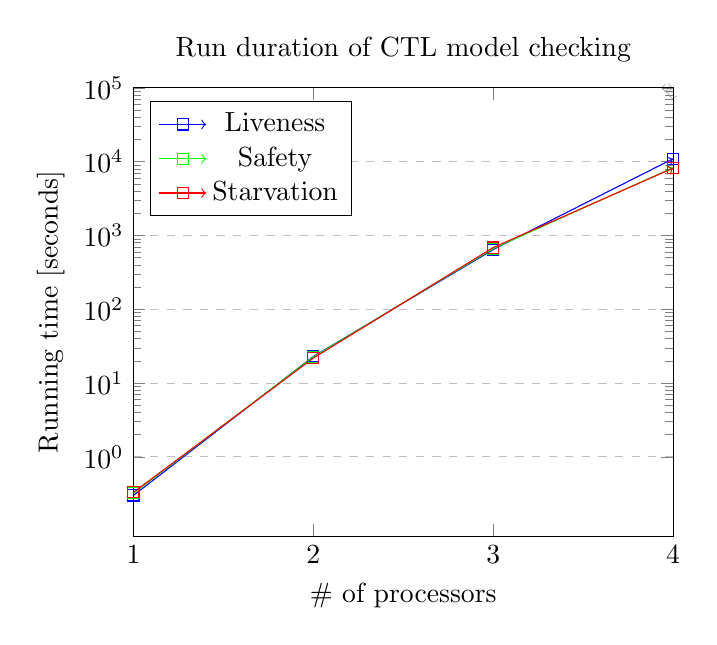
\begin{tikzpicture}
                \begin{semilogyaxis}[
                    title={Run duration of CTL model checking},
                    xlabel={\# of processors},
                    ylabel={Running time [seconds]},
                    xmin=1, xmax=4,
                    ymin=0, ymax=100000,
                    xtick={1,2,3,4},
                    ytick={0,1,10,100,1000,10000,100000},
                    legend pos=north west,
                    ymajorgrids=true,
                    grid style=dashed,
                ]
                 
                \addplot[
                    color=blue,
                    mark=square,
                    ]
                    coordinates {
                    (1,0.3)(2,22.9)(3,644)(4,10961)
                    };
                    \addlegendentry{Liveness}                
                \addplot[
                    color=green,
                    mark=square,
                    ]
                    coordinates {
                    (1,0.32)(2,22.5)(3,665)(4,8301)
                    };
                    \addlegendentry{Safety}
                \addplot[
                    color=red,
                    mark=square,
                    ]
                    coordinates {
                    (1,0.33)(2,21.8)(3,686)(4,8163)
                    };
                    \addlegendentry{Starvation}
                \end{semilogyaxis}
            \end{tikzpicture}
            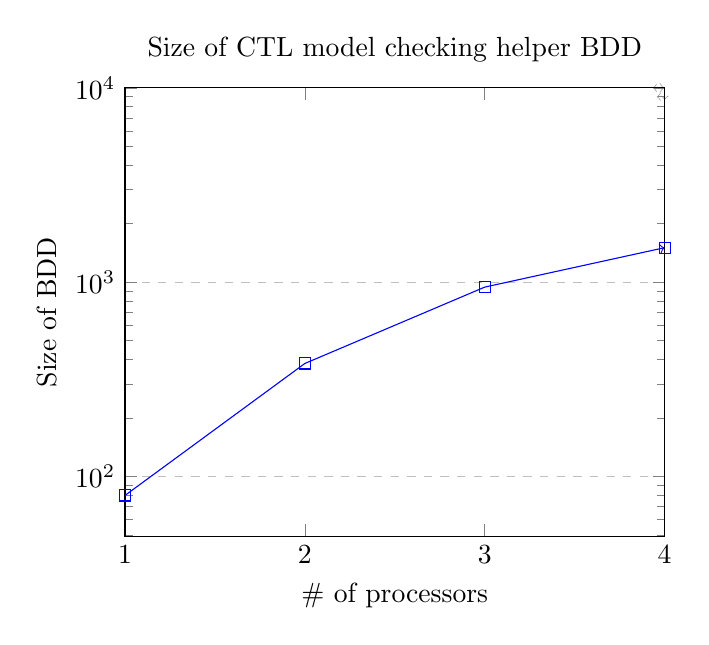
\begin{tikzpicture}
                \begin{semilogyaxis}[
                    title={Size of CTL model checking helper BDD},
                    xlabel={\# of processors},
                    ylabel={Size of BDD},
                    xmin=1, xmax=4,
                    ymin=0, ymax=10000,
                    xtick={1,2,3,4,100},
                    ytick={0,1,10,100,1000,10000},
                    legend pos=north west,
                    ymajorgrids=true,
                    grid style=dashed,
                ]
                 
                \addplot[
                    color=blue,
                    mark=square,
                    ]
                    coordinates {
                    (1,80)(2,382)(3,944)(4,1506)
                    };                    
                \end{semilogyaxis}
            \end{tikzpicture}
        \caption{CTL model checking run stats on models of various sizes} \label{fig:3}
        \end{figure}

    \subsection{Testing the LTL model checker}
        As described in Table 1, the LTL checking computation time is significally longer then the CTL checker. Unfortunately, it
        was so long we could not get any result for models with 3 processors or more. The root of the computation, the SCC finder algorithm,
        took many hours to iterate over the result product model. In this section we will show and briefly discuss the results
        for checking the models with single and two processors.

        The results shown here also compare between the LTL checker with and without simplying the LTL formulas so they only use the $X$ and $U$
        quantifiers. Specifically, the formulas we tested on were:

        \begin{itemize}
            \item Safety
            
            $(1)$ $AG(\lnot sink)$ as oppose to $(1*)$ $A(\lnot (true\ U\ \lnot(\lnot sink)))$

            \item Starvation 
            
            $(2)$ $AG(owned\_waiting \Rightarrow F(owned))$ 
            
            as oppose to 
            
            $(2*)$ $A(\lnot (true\ U\ \lnot(owned\_waiting \Rightarrow true\ U\ (owned))))$
        \end{itemize}

        On section 4.7 we described the actual change in the algorithm needed to compute the tableau for formulas containing the $G$ and $F$
        quantifiers. Considering the quivalences $Fa \equiv true\ U\ a$ and $Ga \equiv \lnot F \lnot a$, theoretically, one can change the appearance
        of each $XF$ and $XG$ elementary formulas with a $XU$ elemntary function, and every fairness constraint with the new kind of fairness constraint
        corresponding to the temporal quantifierts.

        The conversion could help though, mostly because it demands much less computation steps - for example, each computation of sat is completed a bit faster,
        and even the actual formula parsing could be faster (it is much easier to analyze a unary operator string). On figure 4 we show the size of BDD needed to
        present the product of the formula tableau and the model with $n$ processors. Table 2 shows the computation time needed to check the formulas with
        the model of 1 and 2 processors.

        \begin{figure}
            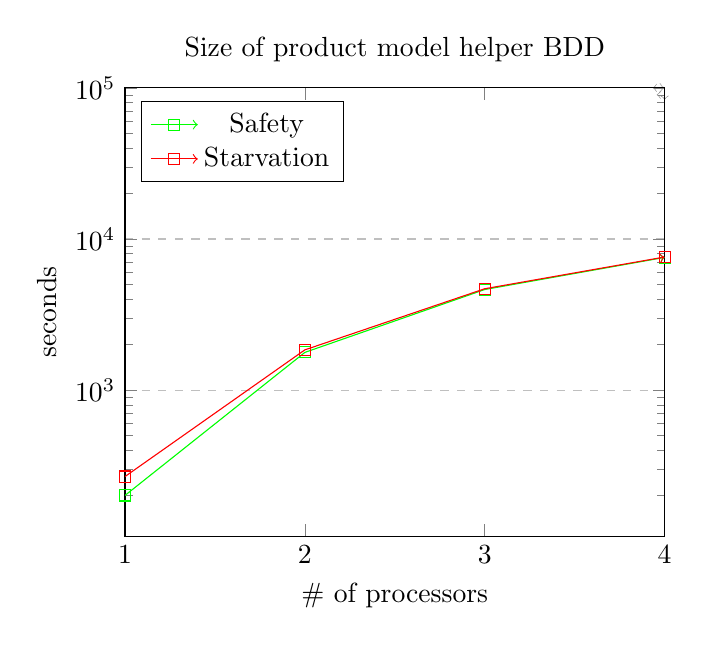
\begin{tikzpicture}
                \begin{semilogyaxis}[
                    title={Size of product model helper BDD},
                    xlabel={\# of processors},
                    ylabel={seconds},
                    xmin=1, xmax=4,
                    ymin=0, ymax=100000,
                    xtick={1,2,3,4},
                    ytick={0,1,10,100,1000,10000, 100000},
                    legend pos=north west,
                    ymajorgrids=true,
                    grid style=dashed,
                ]
                 
                \addplot[
                    color=green,
                    mark=square,
                    ]
                    coordinates {
                    (1,201)(2,1777)(3,4631)(4,7554)
                    };
                    \addlegendentry{Safety}
                \addplot[
                    color=red,
                    mark=square,
                    ]
                    coordinates {
                    (1,268)(2,1847)(3,4687)(4,7601)
                    };
                    \addlegendentry{Starvation}
                \end{semilogyaxis}
            \end{tikzpicture}
            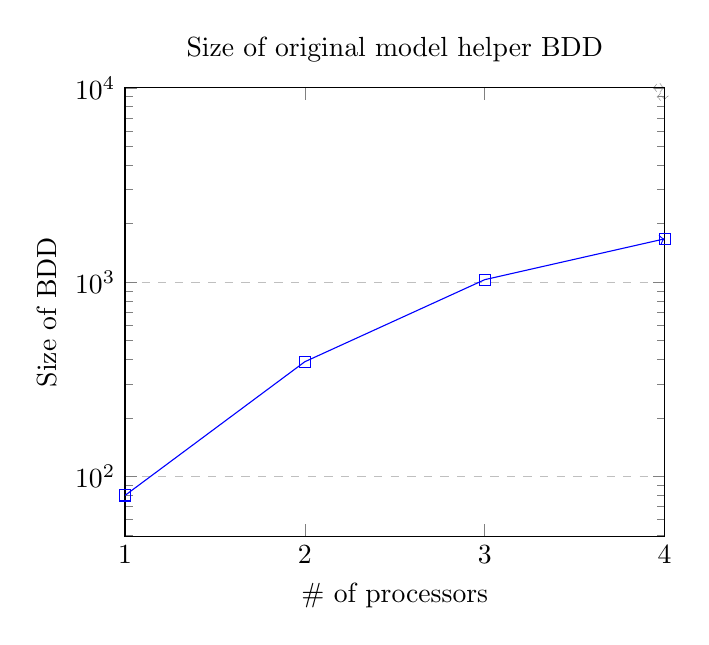
\begin{tikzpicture}
                \begin{semilogyaxis}[
                    title={Size of original model helper BDD},
                    xlabel={\# of processors},
                    ylabel={Size of BDD},
                    xmin=1, xmax=4,
                    ymin=0, ymax=10000,
                    xtick={1,2,3,4,100},
                    ytick={0,1,10,100,1000,10000},
                    legend pos=north west,
                    ymajorgrids=true,
                    grid style=dashed,
                ]
                 
                \addplot[
                    color=blue,
                    mark=square,
                    ]
                    coordinates {
                    (1,80)(2,390)(3,1031)(4,1672)
                    };                    
                \end{semilogyaxis}
            \end{tikzpicture}         
        \caption{State transition for non-master processor (receive a message)} \label{fig:4}
        \end{figure}

        \begin{table}[h!]
        \centering
        \begin{tabular}{||c c c c c||} 
            \hline
            Formula & \# of processors & seconds & size of tableau BDD & \# of SCC found \\ [0.5ex] 
            \hline\hline
            \multicolumn{5}{|c|}{Safety} \\
            \hline
            $(1)$ & 1 & 92 & 215 & 10 \\ 
            $(1*)$ & 1 & 175 & 207 & 10 \\
            $(1)$ & 2 & 7925 & 1768 & 105 \\
            $(1*)$ & 2 & 15459 & 1773 & 105 \\
            \hline
            \multicolumn{5}{|c|}{Starvation} \\
            \hline
            $(2)$ & 1 & 222 & 261 & 17 \\ 
            $(2*)$ & 1 & 435 & 251 & 17 \\
            $(2)$ & 2 & 16327 & 1844 & 196 \\
            $(2*)$ & 2 & 34098 & 1830 & 196 \\
            \hline
        \end{tabular}
        \caption{Results of LTL formula checking on single and two-processor models}
        \label{table:1}
        \end{table}

        As mentioned above, it is clear the computation of the short versions is much faster, even though the size of the tableau stayed about the same (as expected).
        This mostly shows that the overhead of checking the model with the formula takes significant time of the actual computation. Additionally, The number of SCC
        in the product model stays exactly the same between the two versions of formulas. This is because, as established before, the tableau structure stays the same,
        even after using the extended form.

        \begin

\section{Further Work}

    We were surprised by that result - we expected the computation time to be about the same on the simplified. By our analysis this is caused mostly becuase the 
    model building procedure has a significant amount of overhead that is reduced when the formula is less complicated. We tried to reduce that overhead using profiling
    and improving the points of failure in our implementation, without any significant improvements. This is also iteresting because it raises the question how else can we 
    improve the computation so that the LTL model checking is faster. On the other hand, we have established (again) that the LTL model checking is exponential with the size of the model, and that would stay the same, no matter what we find.

\pagebreak
\bibliographystyle{plain}
\bibliography{final_project}

\end{document}
